
%TODO: cite the AST API 


% Many thanks to Andrew West for writing most of this file
% Main LaTeX file for CIS400/401 Project Proposal Specification
%
% Once built and in PDF form this document outlines the format of a
% project proposal. However, in raw (.tex) form, we also try to
% comment on some basic LaTeX technique. This is not intended to be a
% LaTeX tutorial, instead just (1) a use-case thereof, and (2) a
% template for your own writing.

% Ordinarily we'd begin by specifying some broad document properties
% like font-size, page-size, margins, etc. -- We have done this (and
% much more) for you by creating a 'style file', which the
% 'documentclass' command references.
\documentclass{sig-alternate}

% These 'usepackage' commands are a way of importing additional LaTeX
% styles and formattings that aren't part of the 'standard library'
\usepackage{mdwlist}
\usepackage{url}
\usepackage{listings}
\usepackage{float}

\begin{document}
\pagenumbering{arabic}

% We setup the parameters to our title header before 'making' it. Note
% that your proposals should have actual titles, not the generic one
% we have here.
\title{CodeScore}
\subtitle{Dept. of CIS - Senior Design 2013-2014\thanks{Advisor: Chris Murphy (cdmurphy@cis.upenn.edu).}}
\numberofauthors{4}

\author{
	Allison Pearce \\ \email{alpearce@upenn.edu} \\ Univ. of Penn \\ Philadelphia, PA
	\and Spencer Lee \\ \email{lesp@upenn.edu} \\ Univ. of Penn \\ Philadelphia, PA
	\and Tanvir Ahmed \\ \email{tanvir@upenn.edu} \\ Univ. of Penn \\ Philadelphia, PA
\and Will McDermid \\ \email{wmcd@upenn.edu} \\ Univ. of Penn \\ Philadelphia, PA}

\date{}
\maketitle

% Next we write out our abstract -- generally a two paragraph maximum,
% executive summary of the motivation and contributions of the work.
\begin{abstract}
	\textit{The technology industry lacks automated tools for evaluating software
		quality. These tools would be helpful for individuals desiring to improve
		their abilities, recruiters searching for top programmers, and educators
		needing to quickly assess student performance. This work describes
		CodeScore, an application that assesses internal software
	quality by detecting code smells. Code smells are easily recognized design
weaknesses that may indicate more significant problems within the system. The
program recognizes code smells using a set of specific rules that make use of the
abstract syntax of the source code. It then
uses the results to compute a CodeScore: a single value that reflects the
maintainability and understandability of the piece of software based on the
presence of code smells. }
\end{abstract}

% Then we proceed into the body of the report itself. The effect of
% the 'section' command is obvious, but also notice 'label'. Its good
% practice to label every (sub)-section, graph, equation etc. -- this
% gives us a way to dynamically reference it later in the text via the
% 'ref' command.
\section{Introduction}
\label{sec:intro} Software failures result in annoyed users at best, and they can cause
catastrophic system failures at worst. Six people received massive radiation
overdoses from a radiation therapy device in one of the canonical examples of a
fatal software error \cite{leveson1995therac}. Failures are consequences of poor
software quality. Software quality is defined as ``conformance to explicitly
stated functional and performance requirements, explicitly documented
development standards, and implicit characteristics that are expected of all
professionally developed software" \cite{pressman1997}. In addition to causing
failures, disregard for software quality is expensive and inefficient, requiring
more dollars and man-hours to maintain, test, and add features to a project than
should be necessary. An increasing appreciation of well-designed software has
been manifested in the international standard for software quality, ISO/IEC
25010 \cite{iso2011iec}. The standard affirms the importance of specifying and measuring
characteristics of quality, and it defines quality models intended to aid in
accomplishing these goals. 

Software quality is commonly divided into internal quality and external quality.
External quality describes how well the software meets performance expectations,
and encompasses characteristics such as correctness, accuracy, integrity,
robustness, reliability, usability, adaptability, and efficiency. Internal
quality describes how well the software was designed and implemented, and is
concerned with maintainability, flexibility, portability, reusability,
readability, understandability, and testability
\cite{mcconnell1993codecomplete}. Internal and external quality are closely
related, and deficiencies in internal quality lead to deficiencies in external
quality. For example, code that is difficult to understand will also be
difficult to adapt to new requirements, and code that cannot be easily tested
will likely be incorrect or unreliable. 

One way to diagnose internal quality issues is by detecting code smells. Code
smells are easily recognized design weaknesses on the surface of the code that
may indicate deeper, more significant problems within the system. Individual code 
smells are directly related to problems with specific aspects of
internal quality. Examples of code smells include:

\begin{itemize}
	\item Long parameter lists. Large numbers of inputs to a method make the
		code difficult to read, and they make it easy for the programmer to
		introduce a bug by passing in parameters in the wrong order.
	\item Deeply nested conditional logic. A sequence of nested conditionals is
		difficult to understand because the normal path of execution is 
		unclear.
	\item Message chaining (e.g. \texttt{A.getB().getC().getD()}). Message
		chains force class A to depend unnecessarily on classes B and C in order
		to get information from class D. This could introduce complications when any of the
		four classes need to be modified.
	\item Absence of Javadocs. Lack of documentation detracts from
		understandability and maintainability.  
	\item Line length. Lines longer than the standard 80 characters make it
		difficult to read code on smaller monitors.
	\item Method length. Complex, ``do everything" methods are arduous to read and to
		modify. 
	\item Hard coding. Values that are hard coded in multiple places must be
		changed individually by the programmer, which often introduces bugs.
	\item Comment to code ratio. This is another form of documentation that
		should be present in quality code.
\end{itemize}

CodeScore tests for the presence of all of the code smells on the preceding list
in order to evaluate internal quality. The software focuses on code smells that
relate to two
elements of internal software quality: maintainability and understandability.
These elements are underemphasized in most classroom settings. Students work
quickly and haphazardly to meet deadlines and never revisit their programs after
turning them in, so there is no need to write maintainable or understandable code.
However, understandability and maintainability are critical outside of the
classroom, where teams of developers need to understand code they did not write,
and to maintain it for years as the product evolves. CodeScore helps
students assess and improve these necessary software engineering skills by
providing objective feedback to make them aware of their weaknesses. Computer
science teachers can use the the application when grading assignments to assess
quality without spending hours reading through each student's source code. It
also allows recruiters to identify potential employees who will contribute
to their company's products with a high regard for quality at a much lower cost
than most current recruiting practices. Overall, this tool
has the potential to help the technology industry train and recruit a strong developer
workforce who will write programs that are internally sound.

At the core of the program are specific rules for defining code
smells. The rules are used by custom code smell detection algorithms. When a
user uploads their code to be analyzed via the web interface, each detector runs on each file in the
sample. The results of the detections are fed to a scoring module to compute an
internal quality score, the CodeScore, for the piece of software. The CodeScore
and detailed reports with suggestions for improvement are returned to the user.

\section{Related Work}
\label{sec:related_work}
Before describing our methods, we provide background information
on the different methods of analyzing code, the standards for measuring code
quality, and various services and applications that already strive to provide
quantitative analyses of code quality.

\subsection{Code Analysis Methodologies}
The majority of existing applications for measuring code quality rely on
well-established code analysis techniques. These techniques involve breaking
code down into specific units for processing. Such
techniques include parsing the source code into control structures
\cite{mccabe1976complexity}, tokens \cite{halstead1977elements}, assembly
instructions \cite{park1992software}, or objects \cite{chidamber1994metrics}.
Once the source code has been parsed into some unit (this process is called
static analysis), the attributes of the code, such as reliability, security,
efficiency, size, and maintainability can be measured by calculating various
metrics using the parsed results.
The actual approach to measuring these attributes originated in\cite{boehm1976quantitative}
and later became part of the ISO/IEC 25000 series
of standards relating to the quality and evaluation of software
\cite{iso2011iec}. These techniques and standards form the foundation for
today's code quality measurement applications, and they are the basis for our
approach as well.

\subsection{Ohloh}
Launched in January of 2006, Ohloh \cite{allen2009ohloh} is web service and
online community owned by Black Duck Software which provides basic metrics for
over 650,000 open source projects containing over 24 billion lines of code
located in over 620,000 source code repositories and managed by more than
3,000,000 contributors. These projects are retrieved from source control
repositories and analyzed. Metrics such as lines of code, amount of source code
comments, and estimated software cost (based on the COCOMO model
\cite{boehm2000software}) are provided, along with commit statistics, project
activity, and programming language detection. This data is graphically displayed
when one views a project's information on the site. Ohloh also provides global
statistics across all projects for different programming languages and
contributor statistics for different authors of open source code. 

Ohloh primarily focuses on tracking project/contributor activity for large
open-source projects. CodeScore focuses more on providing code quality-oriented
metrics.

\subsection{Common Weakness Enumeration}
The Common Weakness Enumeration (CWE) \cite{mitre2006cwe} is a
community-developed list of software weaknesses hosted by the MITRE Corporation.
The CWE was developed with the intention of providing:

\begin{itemize}
	\item a common standard of identifying, mitigating, and preventing software weaknesses.
	\item a common source of measuring weaknesses for software security tools.
	\item a common language for describing the various types of software
		weaknesses that exist in computer architecture, software design, and
		source code.
\end{itemize}

CWE supports the discovery of common types of software security flaws such as
buffer overflows, handler errors, pathname traversals, and resource management
errors (amongst others) within code.

%CWE began with the Common Vulnerabilities and Exposures (CVE) list in 1999 \cite{mitre2005cve}. As part of the SAMATE project \cite{nist2005samate}, MITRE later expanded upon the CVE list with the Preliminary List of Vulnerability Examples for Researchers (PLOVER) \cite{christey2005plover}. PLOVER was the first attempt to take real-world examples of software vulnerabilities and abstract them into common classes of more general vulnerabilities that can arise during the software development process. The goal of PLOVER was to make this information available to developers, researchers, and analysts so that they may use it for a variety of purposes, with the goal of improving code security. CWE encompasses much of the CVE list and expands upon PLOVER by establishing community-developed definitions and descriptions of these common weaknesses.

The Preliminary List of Vulnerability Examples for Researchers, or PLOVER~\cite{christey2005plover},
was an early form of CWE. PLOVER was the first attempt
to take real-world examples of software vulnerabilities and abstract them into
common classes of more general vulnerabilities that can arise during the
software development process. The goal of PLOVER was to make this information
available to developers, researchers, and analysts so that they may use it with
the goal of improving code security. CWE expands upon PLOVER by establishing
community-developed definitions and descriptions of these common weaknesses.

CWE primarily strives to provide standards relating to the weaknesses of code in
terms of security. This may be a valuable resource as we develop additional features for
CodeScore, as many security weaknesses are indicative of, or are themselves, code 
smells, but our project has a wider scope. CWE also incorporates community feedback in
developing definitions of weaknesses, which is a strategy we also intend to use
in verifying and fine-tuning our models.

\subsection{HIST}
Historical Information for Smell deTection, or HIST \cite{palomba}, is an
approach developed to detect five specific code smells using change history from
version control systems.  The developers of HIST point out that not all code
smells are possible to detect using just source code because some are by
definition characterized by how the code changes during the project's
development. One example is parallel inheritance hierarchies, in which ``every
tme you make a subclass of one class, you have to make a subclass of another"
\cite{fowler1999}. Though revision histories often display changes at a
file-level granularity, they use a tool called the Change History Extractor to parse
changes at a method- and class-level granularity, and then they identify code 
smells from the parsed logs using specific rules. CodeScore will soon
make use of a similar strategy for incorporating version control information
into several metrics, but CodeScore's analysis includes many more metrics than just
those that can be detected using revision logs.

\begin{figure*}[ht]
	\begin{center}
		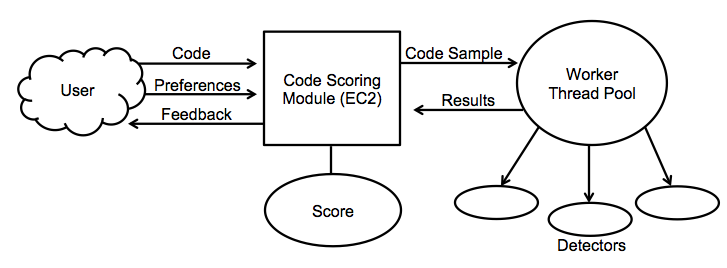
\includegraphics[width=0.9\linewidth]{block_diagram}
	\end{center}
	\vspace{-12pt}
	\caption{System architecture}
	\label{fig:some_graph}
\end{figure*}

\subsection{JOCS}
Judgment of Code Style (JOCS) was a CIS 400/401 project in the 2012-2013
academic year \cite{close2013jocs}. Their goal was to create a tool for an automated
analysis of code style. Such a tool would be useful in assigning the style grade
often associated with assignments in introductory programming classes, such as
CIS 110 or 120 at the University of Pennsylvania. Features of interest included
line length, modularity, and consistency. They used machine learning to compute
a single score from the features. CodeScore will make use of similar techniques,
but the two projects will be using mostly non-overlapping feature sets and
different strategies for identifying them. Our focus is not on style but on code
smells as they relate to internal quality, which ultimately affects the
correctness, efficiency, and overall external quality of the program. 

\subsection{Other Static Code Analysis Tools}
A wide variety of other static code analysis tools also exist, including
CodeSonar~\cite{grammatech2013codesonar}, KlocWork Insight~\cite{klocwork2013insight},
FindBugs~\cite{pugh2013findbugs}, and Yasca~\cite{scovetta2007yasca}. These
applications focus mostly on external quality metrics such as security,
reliability, correct functionality, and efficiency. Most can be used with a variety of
programming languages and offer reports or visualizations of the results.

CodeScore offers a novel solution amongst all of these existing tools.
While most of the current applications are principally concerned with external
quality, our tool focuses on internal quality. Internal quality has a strong
correlation with external
quality, so writing code with an emphasis on internal quality allows developers
to spend less time testing and fixing bugs and
more time on new products and features. Additionally, many existing tools
target industry developers, but one of our primary target audiences is
students. Students need to develop an appreciation for internal quality
before entering the workforce or academia, but these skills are often
underemphasized at the undergraduate level. Finally, our solution attempts to
provide more functionality than the majority of similar open-source
applications. CodeScore aims to provide quality of functionality similar to
commercial-grade applications in a form that is accessible to a wider
audience.

\section{System Model}
\label{sec:system_model}
%TODO put code smells in this section

%CodeScore quantitatively assesses code
%quality. It is an objective tool for performing a task that seems inherently
%subjective. The characterization of software quality has been the topic
%of much discussion in both academia in industry. Using as a foundation the
%components of internal quality described in \cite{iso2011iec} and similar
%reports, our program further dissects these components into specific patterns
%that can be identified in source code. The holistic scoring system is built up
%from a large collection of these specific, detectable indicators to provide one
%comprehensive measure of quality.

CodeScore focuses on evaluating internal quality, and as such primarily uses static code
analysis techniques. This allows for the assessment of source code without bias from different
system architectures or environments. Code smells provide a powerful but simple
indicator of internal quality because they are specific and detectable, and they
have a clear relationship with internal quality. The
program currently focuses on understandability and maintainability. 

\emph{Understandability} is a measure of how easy a code sample is for a human to
interpret. It can be estimated in part by the length of message chains (a code
smell in which one method invokes another, which invokes another, and so on in a
long one-line sequence of function calls), length of parameter lists, by
determining what fraction of variable names are dictionary words versus strings
of letters and numbers, and by analyzing the class structure of a program. 

\emph{Maintainability} is a measure of how easy a code sample will be to update
and change. It can be estimated in part by detecting and recognizing coupling
between classes, duplicated code, classes and methods that are too large, and
hard coding. 

CodeScore implements the workflow illustrated in Figure~\ref{fig:some_graph}. The
key components of the system are the main driver and thread pool, the detectors,
and the scoring module. CodeScore includes detectors for the following code smells: 
\begin{itemize}
	\item Long parameter lists. This smell is detected by identifying method
		declarations and counting the number of parameters in the signature. The
		maximum allowable parameter list length can be configured by the user.
	\item Deeply nested conditional logic. This smell is detected by identifying
		conditional statements and determining if they contain additional conditional
		statements within the blocks of code that are entered if a particular
		condition is met. The level of nesting considered acceptable can be
		configured by the user.
	\item Message chaining. This is detected by identifying all method
		invocations and determining if the calling object of the method is
		itself a method invocation. Note that it is not sufficient
		simply to detect methods that appear in the same line, because then an
		expression such as: \begin{verbatim}System.out.println("x is: " + x.get() + " and y
		is: " + y.get());\end{verbatim} would be incorrectly labeled a message
		chain.
	\item Absence of Javadocs. This is detected by identifying Javadocs and
		comparing the ratio of the number of methods and classes declared in the software 
		to the number of Javadocs. 
	\item Line length. This is detected by counting the number of characters in
		each line.
	\item Method length. This is detected by counting the number of lines of
		code (not including white space or comments) in a method declaration.
	\item Hard coding. This is detected by identifying literals (for example, string
		literals or integer literals). The detector then determines if the
		literals are being used in an acceptable context, such as a variable assignment, 
		annotation, or in a statement such as \texttt{return true;}, or if
		they are hard-coded values.
	\item Comment to code ratio. This is detected by differentiating between
		lines of comments, lines of code, and blank lines, then counting the instances of each.
\end{itemize}

The detectors are the most complicated component of the system and present the
greatest technical challenges. Each code smell requires a unique detection
algorithm, sometimes involving analysis of multiple classes together or complex
parsing. The detectors search for all possible patterns indicative of a
particular code smell using the syntactical structure of the program. They track the number and location of all 
violations, compiling them into comprehensive reports in javascript object notation (JSON) for interpretation by
other modules in the system. In detectors which equire thresholds, 
such as the maximum depth allowed for nested conditionals, the program's default
parameters can be overriden by inputting custom parameters.

Users access CodeScore using a web application that provides a platform for
developers to assess and showcase their abilities and for recruiters to identify
promising candidates. Developers can create an account
and upload their projects for analysis. Processing occurs with the detectors
running in parallel, and once completed, a report
provides the overall CodeScore for the project, which is a grade out of 100
points that is analogous to a grade on an essay. It also shows the subscores of each
individual file in the project, graphs displaying the frequency of violations
for each metric, and specific suggestions for improvement that include line
numbers and snippets from the user's code. This report can be shared as a quick and objective
evaluation of one's programming ability, used as a tool for
self-improvement, or incorporated into teachers' grading rubrics. The app also charts CodeScores for revisions
of projects that are uploaded for re-assessment so that the user can track
improvement over time.

The interface for recruiters focuses on searching for and finding information
about talented programmers. When viewing a candidate, recruiters can see the candidate's average
CodeScore and ranking as compared to other users. They can also view the
candidate's education history, previous employers, answers to sample behavioral
questions, and a project showcase. 

\section{System Implementation}
\label{subsec:approach}

All processing for CodeScore happens on an Amazon EC2 cloud processing machine.
EC2 is a service that provides resizable computing capacity in the cloud. 
Users upload Java code in the form of a single .java file or a zip file under
10MB in size containing one or more .java files and a preferences file to the EC2 instance through our website, which
we developed in PHP. The software ensures that the uploaded project is not
malicious using basic validation techniques that search for traits that exist in
malware (e.g. known checksums or invalid filetypes). After passing validation,
the upload is indexed on Amazon S3. S3 stands for Simple Storage Service and is
a component of the Amazon AWS suite of web services. After indexing, the server
launches a process that scans for all appropriate files (Java files or
preferences files) and saves some of the metadata to include in the report. The preferences 
file is encoded in JSON and includes information that is specific to each detector, 
such as thresholds for certain code smells. It also includes optional weights if
the user would like to change how much a given detector influences the overall
CodeScore. A sample preferences file can be
seen in Figure \ref{fig: json}. If no preferences
file is included, the program only runs using the default values. If a
preferences file is included, the program runs once with the default settings to
compute a standard CodeScore used to compare the user with other registered candidates and
once with the custom settings. 

\begin{figure}[ht]
	\begin{center}
		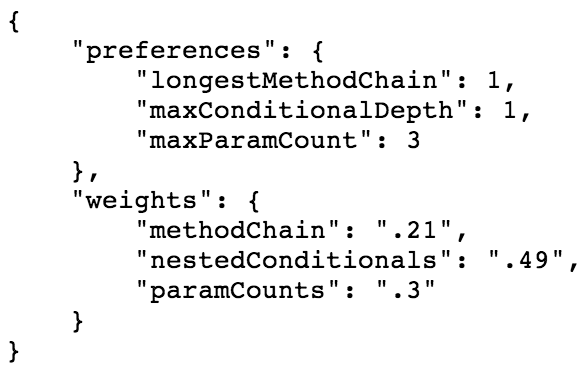
\includegraphics[width=0.9\linewidth]{json}
	\end{center}
	\vspace{-12pt}
	\caption{User preferences file encoded in JSON}
	\label{fig: json}
\end{figure}

When software is uploaded to the endpoint, the controller class
generates $n$ worker threads, where $n$ is the number of detection algorithms to be
performed on the software sample. Currently, $n=8$ because the program supports $8$
different detectors. Each of the workers performs a specific detection task on
each uploaded file and then sends results back to the scoring module. The
type of result reported to the scoring module depends on the detector, but in
most cases the detector reports a count of the number of violations of that
metric in each file normalized to a percentage between zero and one hundred. The
percentage represents how acceptable the file is with regard to that particular
code smell, taking into account the length of the file and the number of
violations. 

The scoring module combines all of the normalized detector outputs into a
weighted average representing the subscore for a particular file. Some detectors
are weighted more heavily than others. These weights are based on experiments
and user surveys. The subscores for each file are combined into the final
CodeScore. Each file is weighted by importance, considering factors such as the
number of lines it contributed to the project and the number of times methods or
objects from that file are used throughout the project. The end result of this 
process is a single score that gives a user an at-a-glance measure of the internal quality of a project.
The web application also provides more detailed feedback using
HighCharts~\cite{highcharts} , a
JavaScript framework used for making graphs online. Users can navigate to view
reports for a specific file or a general overview.

\begin{figure*}[ht]
	\begin{center}
		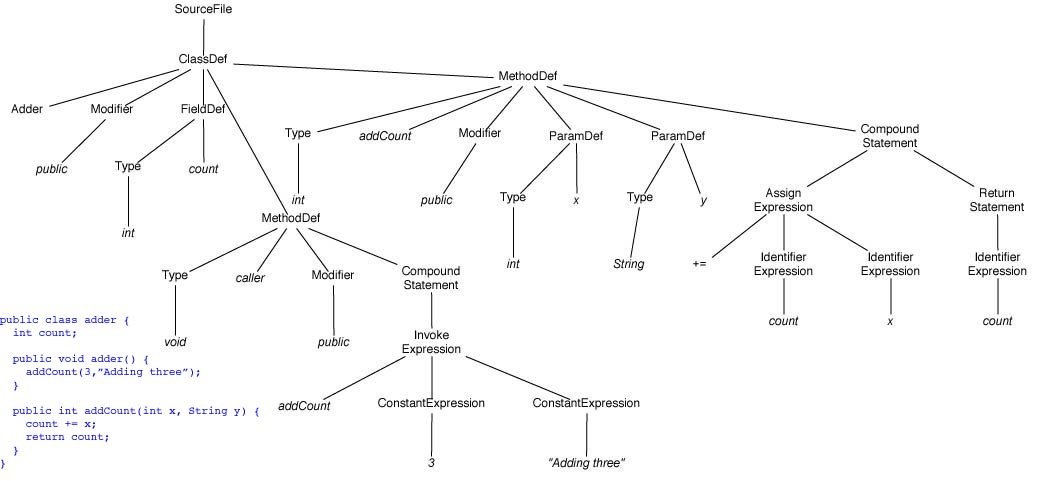
\includegraphics[width=0.9\linewidth]{syntax_tree}
	\end{center}
	\vspace{-12pt}
	\caption{Sample Java abstract syntax tree}
	\label{fig: ast}
\end{figure*}

The program controller, scoring module, and all detectors are implemented in
Java. Multithreading and concurrency of the detectors is accomplished Java's threading libraries
and a custom worker thread pool. The detection algorithms use the Eclipse Java Abstract 
Syntax Tree (AST) API to parse the
Java code as a first step in finding code smells. Traversing the AST allows the
system to access and manipulate Java code at the syntactic level, efficiently searching
for specific elements such as if statements or method invocations. The AST API also
provides information about the location of a particular expression within the
tree, both in terms of line numbers and in terms of the surrounding code.  
Though CodeScore only supports Java at this time, detecting code smells at the AST level 
makes the program easy to adapt to additional programming languages in the future.
Most object-oriented code smells have the same properties from the perspective of the AST,
which abstracts away the specifics of individual programming languages. A sample
abstract syntax tree and the Java code it represents can be seen in Figure~\ref{fig: ast}.

The web application (techruit.me) is implementented in PHP and makes use of search engine
optimization techniques. Custom PHP scripts generate page content, comment, and optimize
formatting for each view on the website. The website is also integrated with
social media using Facebook's Open Graph tags. This allow the page to be liked and shared on
Facebook and provides information to other users when the page receives
attention. Several screenshots of the web application can be seen in Appendix
A.

\begin{figure*}[ht!]
	\begin{center}
		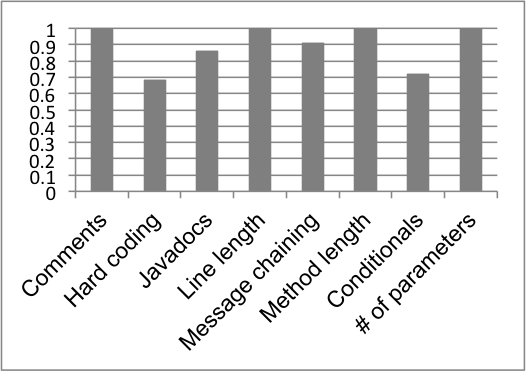
\includegraphics[width=220px]{accuracy}
	\end{center}
	\vspace{-12pt}
	\caption{Detector Accuracy}
	\label{fig: acc}
\end{figure*}


Efficiency is a challenge that is critical to the usefulness of the CodeScore
platform. CodeScore is designed to run
on large and small software projects, which means that all parsing, processing,
and reporting must be carefully engineered to produce results in a timely
manner. CodeScore employs parallel processing techniques so that the runtime
scales well with the number of metrics and the size of the input.

One drawback of the overall CodeScore system is that it is largely centralized.
If the server containing the controller code is compromised at any time during
the computation, all progress in the analysis will be lost. A possible future development
is to decentralize the process so that loss of a server does
not result in complete loss of progress. Ideally, this could be implemented
using MapReduce \cite{dean2008mapreduce}.

\section{Results}

CodeScore has been evaluated on four main criteria:

\begin{itemize}
	\item How accurately code smells are detected.
	\item How the CodeScore compares to human grading.
	\item How quickly the analysis is completed.
	\item The success of the website.
\end{itemize}

For the first criterion, we designed user surveys in which users identified
the same code smells that are detected by CodeScore. For testing small projects,
we asked three volunteers to write short Java programs (100-300 lines of code) 
that included some examples of what they considered ``bad code." For medium-sized
projects (500-1000 lines of code), we used assignments submitted by
randomly selected students in CIS 120 at the University of Pennsylvania. Finally, to test larger
projects, we used open-source Java projects publicly hosted on Github (>2000
lines of code). Each participant evaluated one
code sample of each size in three separate sessions for a total of nine code
samples per person. Participants were given a list of the code smells, their
definitions, and examples, and asked to identify all instances of them in the
provided code samples. We considered a code smell
``detected" by the participants if at least one third of them (9 people) marked the same
line. Figure~\ref{fig: acc} displays the percentages of code smells correctly
identified by the CodeScore detectors as compared to human identification in the
user studies. 

CodeScore detected $100\%$ of violations using the comment to code ratio, line
length, method length, and number of parameters detectors. The absence of
Javadocs and message chaining detectors were both over $80\%$. The detectors
for nested conditionals and hard coding are the most technically challenging,
which is reflected in their accuracy performance ($72\%$ and $68\%$,
respectively). False positives were not an issue with any detectors except for
hard coding.

To compare CodeScore's final grade to the grade a human would assign, we also asked study
participants to assign a score from 0 to 100 to each piece of code they analyzed. We used
feedback from the first session to fine-tune the weights of the detectors used
in calculating the CodeScore. We found that the CodeScore assigned by the
software was within $14\%$ of the average score assigned by the study
participants for five of the six code samples assessed in the second and third
sessions.  

To analyze runtime, we pulled additional open source projects with up to
10,000 lines of code to use as inputs to the system. Projects of this size were not feasible to ask user study
partipants to analyze in the detector and scoring accuracy studies, but they were informative for collecting runtime information. The speed of execution varied roughly linearly with the number of lines of code in
preliminary tests. The bottleneck in runtime seems to be the Java Abstract
Syntax Tree API. However, the benefits of using the AST API in terms of simplicity and
modularity outweigh the slight slowness in processing. See Figure~\ref{fig:runtime} for a graph of the runtime analysis results.

The success of the web application can be quantified using search results and various analytics
provided by Google. At the time of publishing of this report, the website (techruit.me) ranks in 
the top two results when searching Google for ``techruit". The website is in the
top 8 results on
Google and top 4 on Bing when the search term is ``codescore recruiting." The
landing page received over 2,000 pageviews during the time of development, which
is highly promising considering that there was no formal marketing. The bounce
rate, or the number of users who are interested enough to view other pages after
the landing page, is about $50\%$. About $10.5\%$ of users continue to look at
the developers portal and $8.3\%$ look at the recruiters portal.


\begin{figure}[ht]
	\begin{center}
		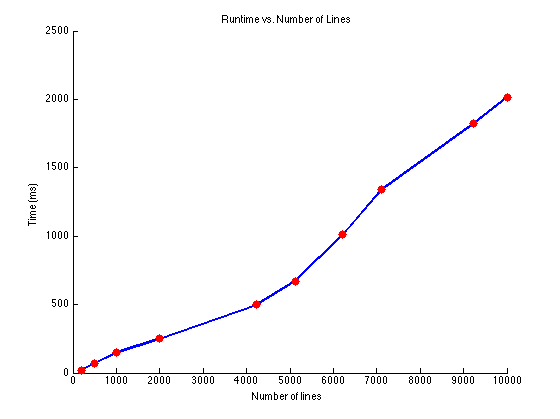
\includegraphics[width=250px]{runtimePlot}
	\end{center}
	\vspace{-12pt}
	\caption{Preliminary Runtime Analysis of CodeScore Module}
	\label{fig:runtime}
\end{figure}

\section {Future Work}
Moving forward, there are a number of interesting questions to be investigated
with CodeScore. An obvious improvement is to add support for other programming
languages in addition to Java. Because CodeScore uses the Java Abstract Syntax
Tree API to parse the source code, most of the language-specfic considerations
have been abstracted away. The detectors look for patterns that are considered
detrimental to internal quality in any object-oriented language. Therefore, adding new programming
languages that have existing APIs for their syntax trees would simply be a
matter of plugging in the new API. A more difficult problem is to include other
programming paradigms, such as functional programming.

Even within the realm of Java and object-oriented programming, there are
enhancements that could help CodeScore perform a more thorough assessment of
internal quality.
Certain code smells, such as shotgun surgery, cannot be detected using just the
source code. Shotgun surgery describes the situation in which making one
change in behavior requires modifying the code in several places. For
example, if logging statements are implemented separately in each function in a
class, then adding line numbers to the logs will require considerable time and effort. A
better solution would be to write a log wrapper for all of the functions, so
that any changes only need to be made once. 
Using
revision history, detecting code smells like shotgun surgery is possible. Analyzing revision
history requires a custom parser that can extract changes at method-level
granularity in order to determine which methods are changing together. Using
revision history might also make it possible to analyze collaborative projects
and score each contributor based only on the code that he or she wrote. After
creating such a parser and adding the corresponding analyses to the program, it 
would be simple to link the CodeScore web application to Github and pull entire repositories,
including git logs, for processing. 

\section{Ethics}
CodeScore raises few ethical questions. The most significant ethical issue with CodeScore is the possibility of
misleading potential employers. If the software were to be adopted by companies to aid in
their hiring procedures, and if flaws in the system made it appear that a particular
programmer was less qualified than he or she really was, that person might not be
hired. CodeScore would be at least partially responsible for keeping that individual 
from finding work. It is also possible that the opposite could occur - CodeScore
might lead to someone being hired despite being underqualified. If the person
broke something critical, such as the Apple developer who introduced the ``goto
fail" bug, CodeScore might also be partially responsible.  Other than these
scenarios or a similar situations, however, the software presents no
major ethical issues. There is almost no physical, financial, or emotional risk to
users.

\section{Conclusions}
CodeScore is a program that performs an automated assessment of the internal
quality of a piece of software. The code is graded based on the presence of 
specific code smells that detract from the maintainability and understandability
of software. Code smells are detected using custom algorithms, and the results of these algorithms are
used to compute a single numerical score (the ``CodeScore") for the software.
The score provides a quick, easy-to-understand measure of the internal quality
of the project. The program also provides detailed reports and suggestions for improvement. Of the eight
detectors, six achieved over $80\%$ accuracy, and the CodeScore itself was shown
to be highly correlated with grades assigned by participants of user studies. CodeScore is useful for
individuals who want to improve their abilities, recruiters seeking an
inexpensive way to assess potential hires, and instructors who want to reinforce
the importance of writing quality code. CodeScore is part of an online platform that allows
developers to assess and optionally showcase their code and
helps connect recruiters with talented programmers. 
% We next move onto the bibliography.
\bibliographystyle{plain} % Please do not change the bib-style
\bibliography{main}  % Just the *.BIB filename

% Here is a dirty hack. We insert so much vertical space that the
% appendices, which want to begin in the left colunm underneath
% "references", are pushed over to the right-hand column. If we looked
% hard enough, there is probably a command to do exactly this (and
% wouldn't need tweaked after edits).
\vspace{175pt}
\appendix
\section{Web Application Screenshots}
\begin{figure}
	\begin{center}
		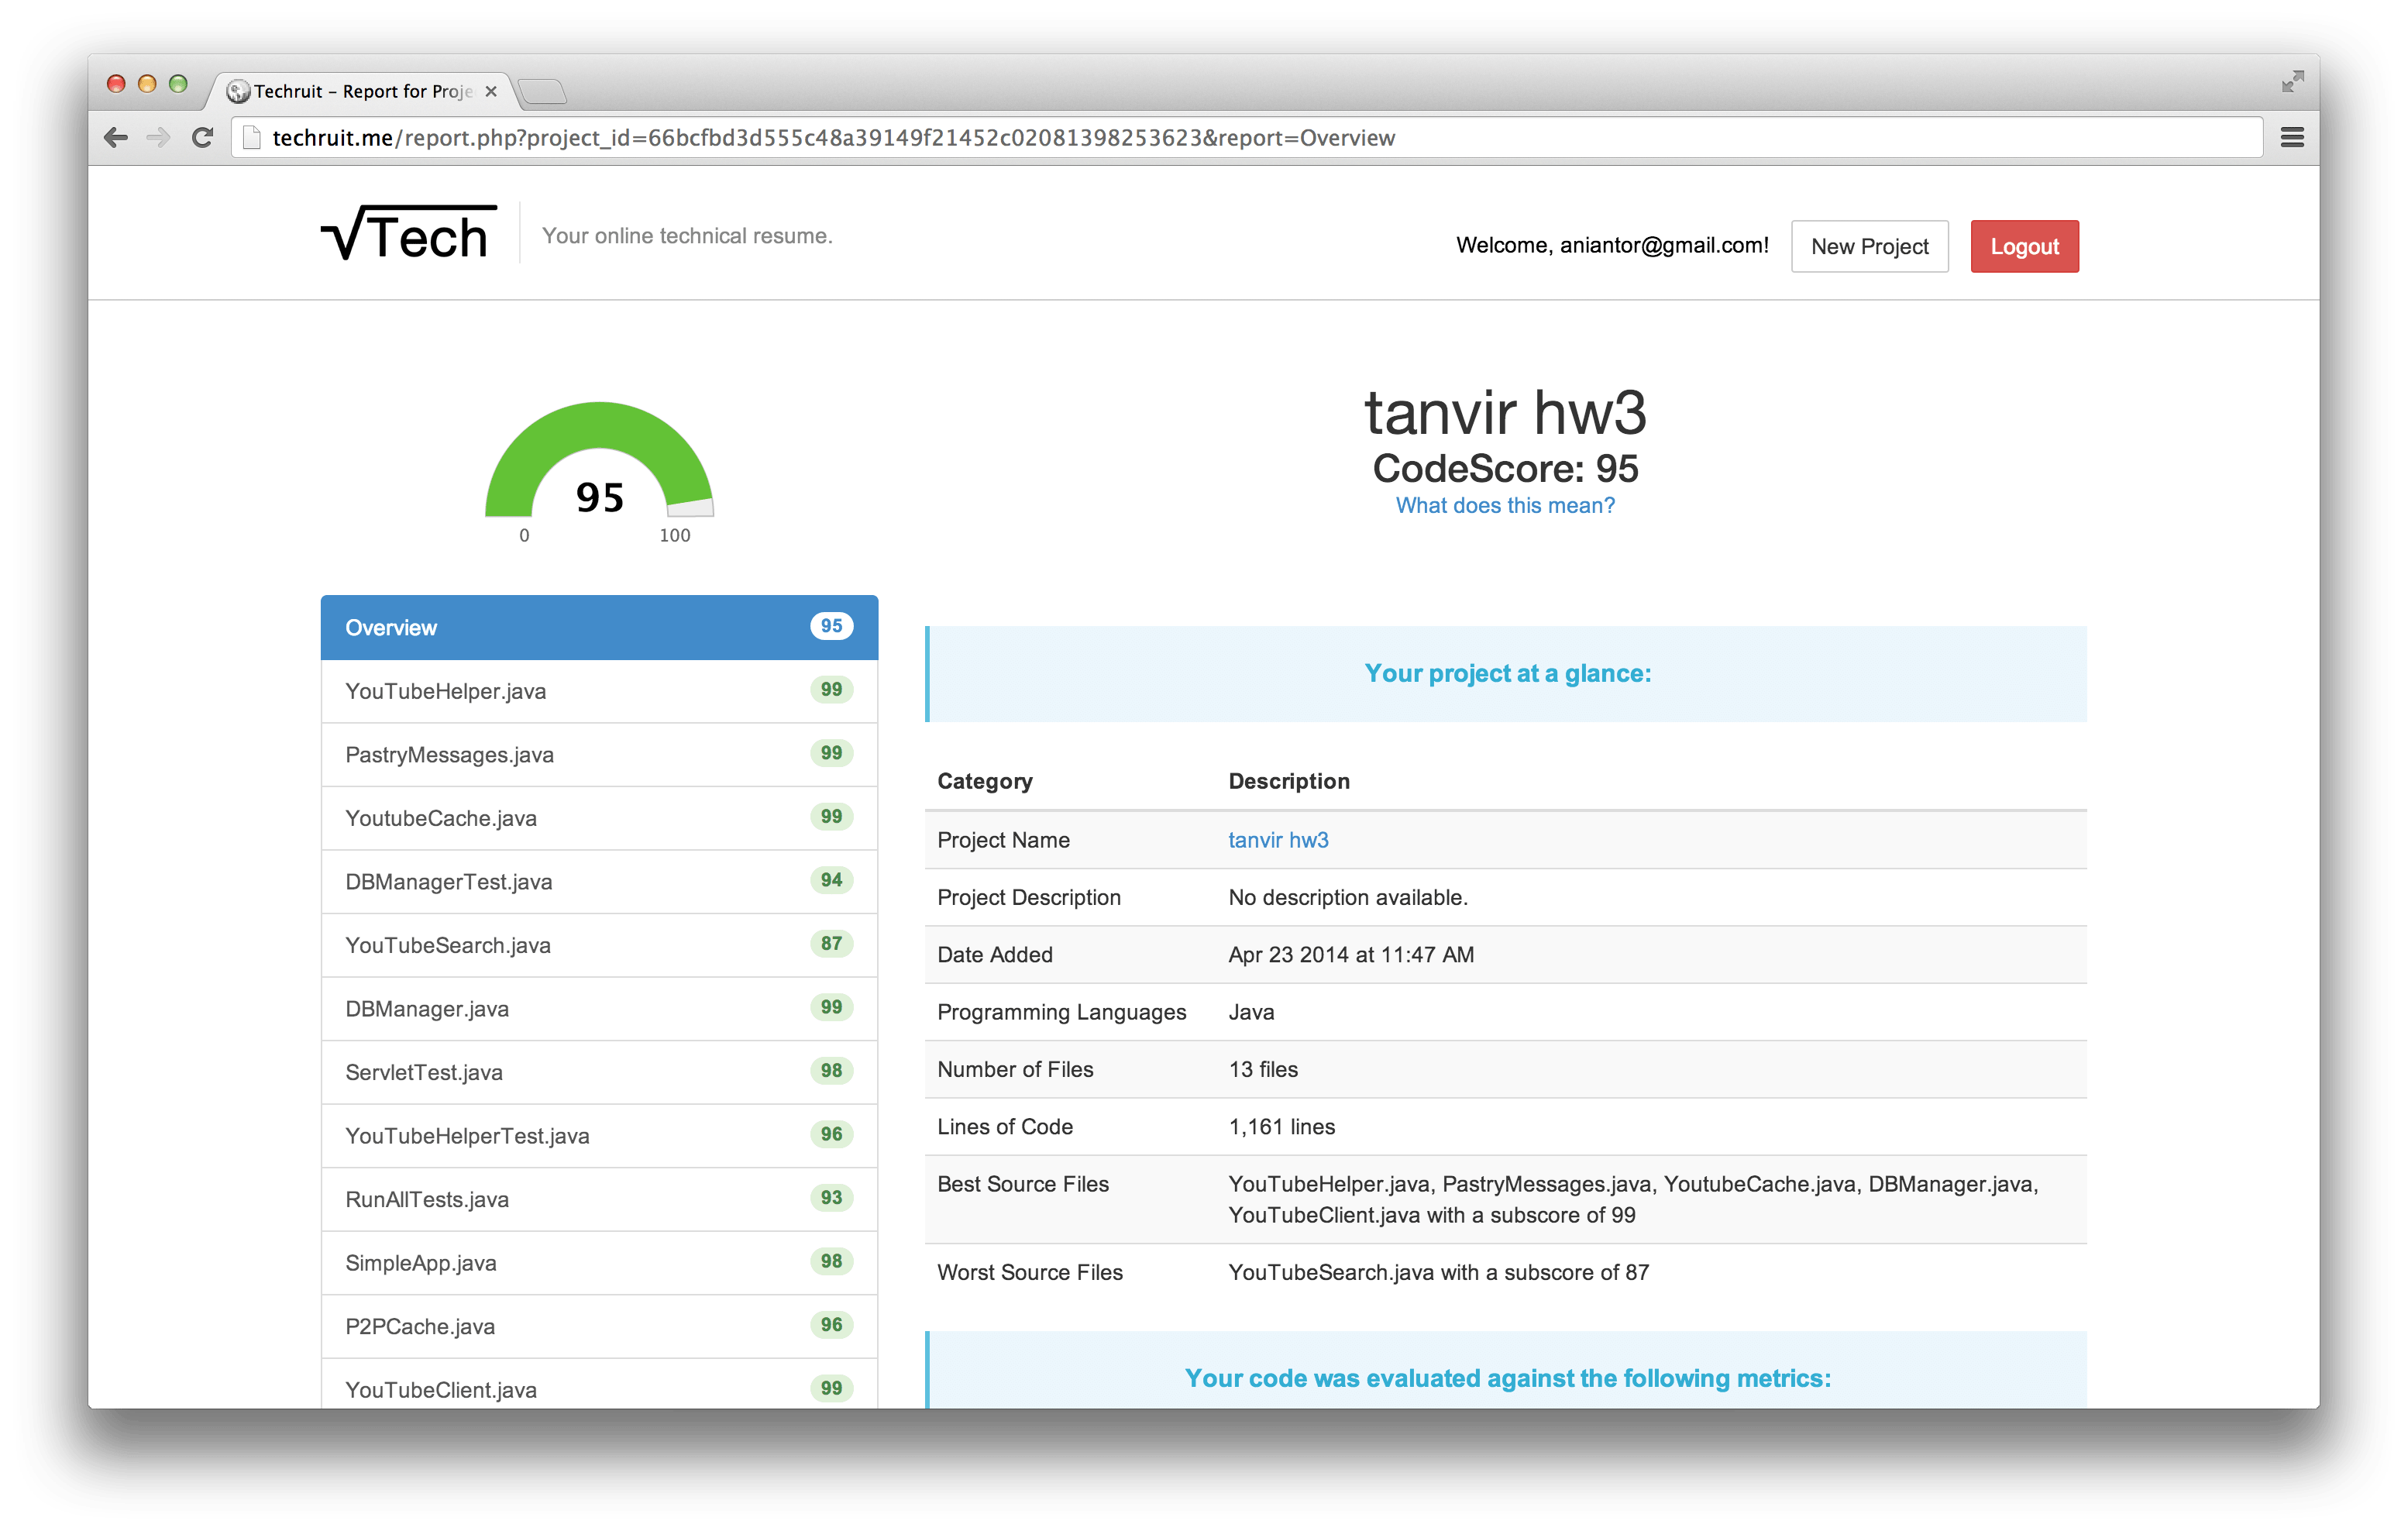
\includegraphics[width=500px]{report_overview1}
	\end{center}
	\vspace{-12pt}
	\caption{Top of Report Page}
	\label{fig:report1}
\end{figure}

\begin{figure}
	\begin{center}
		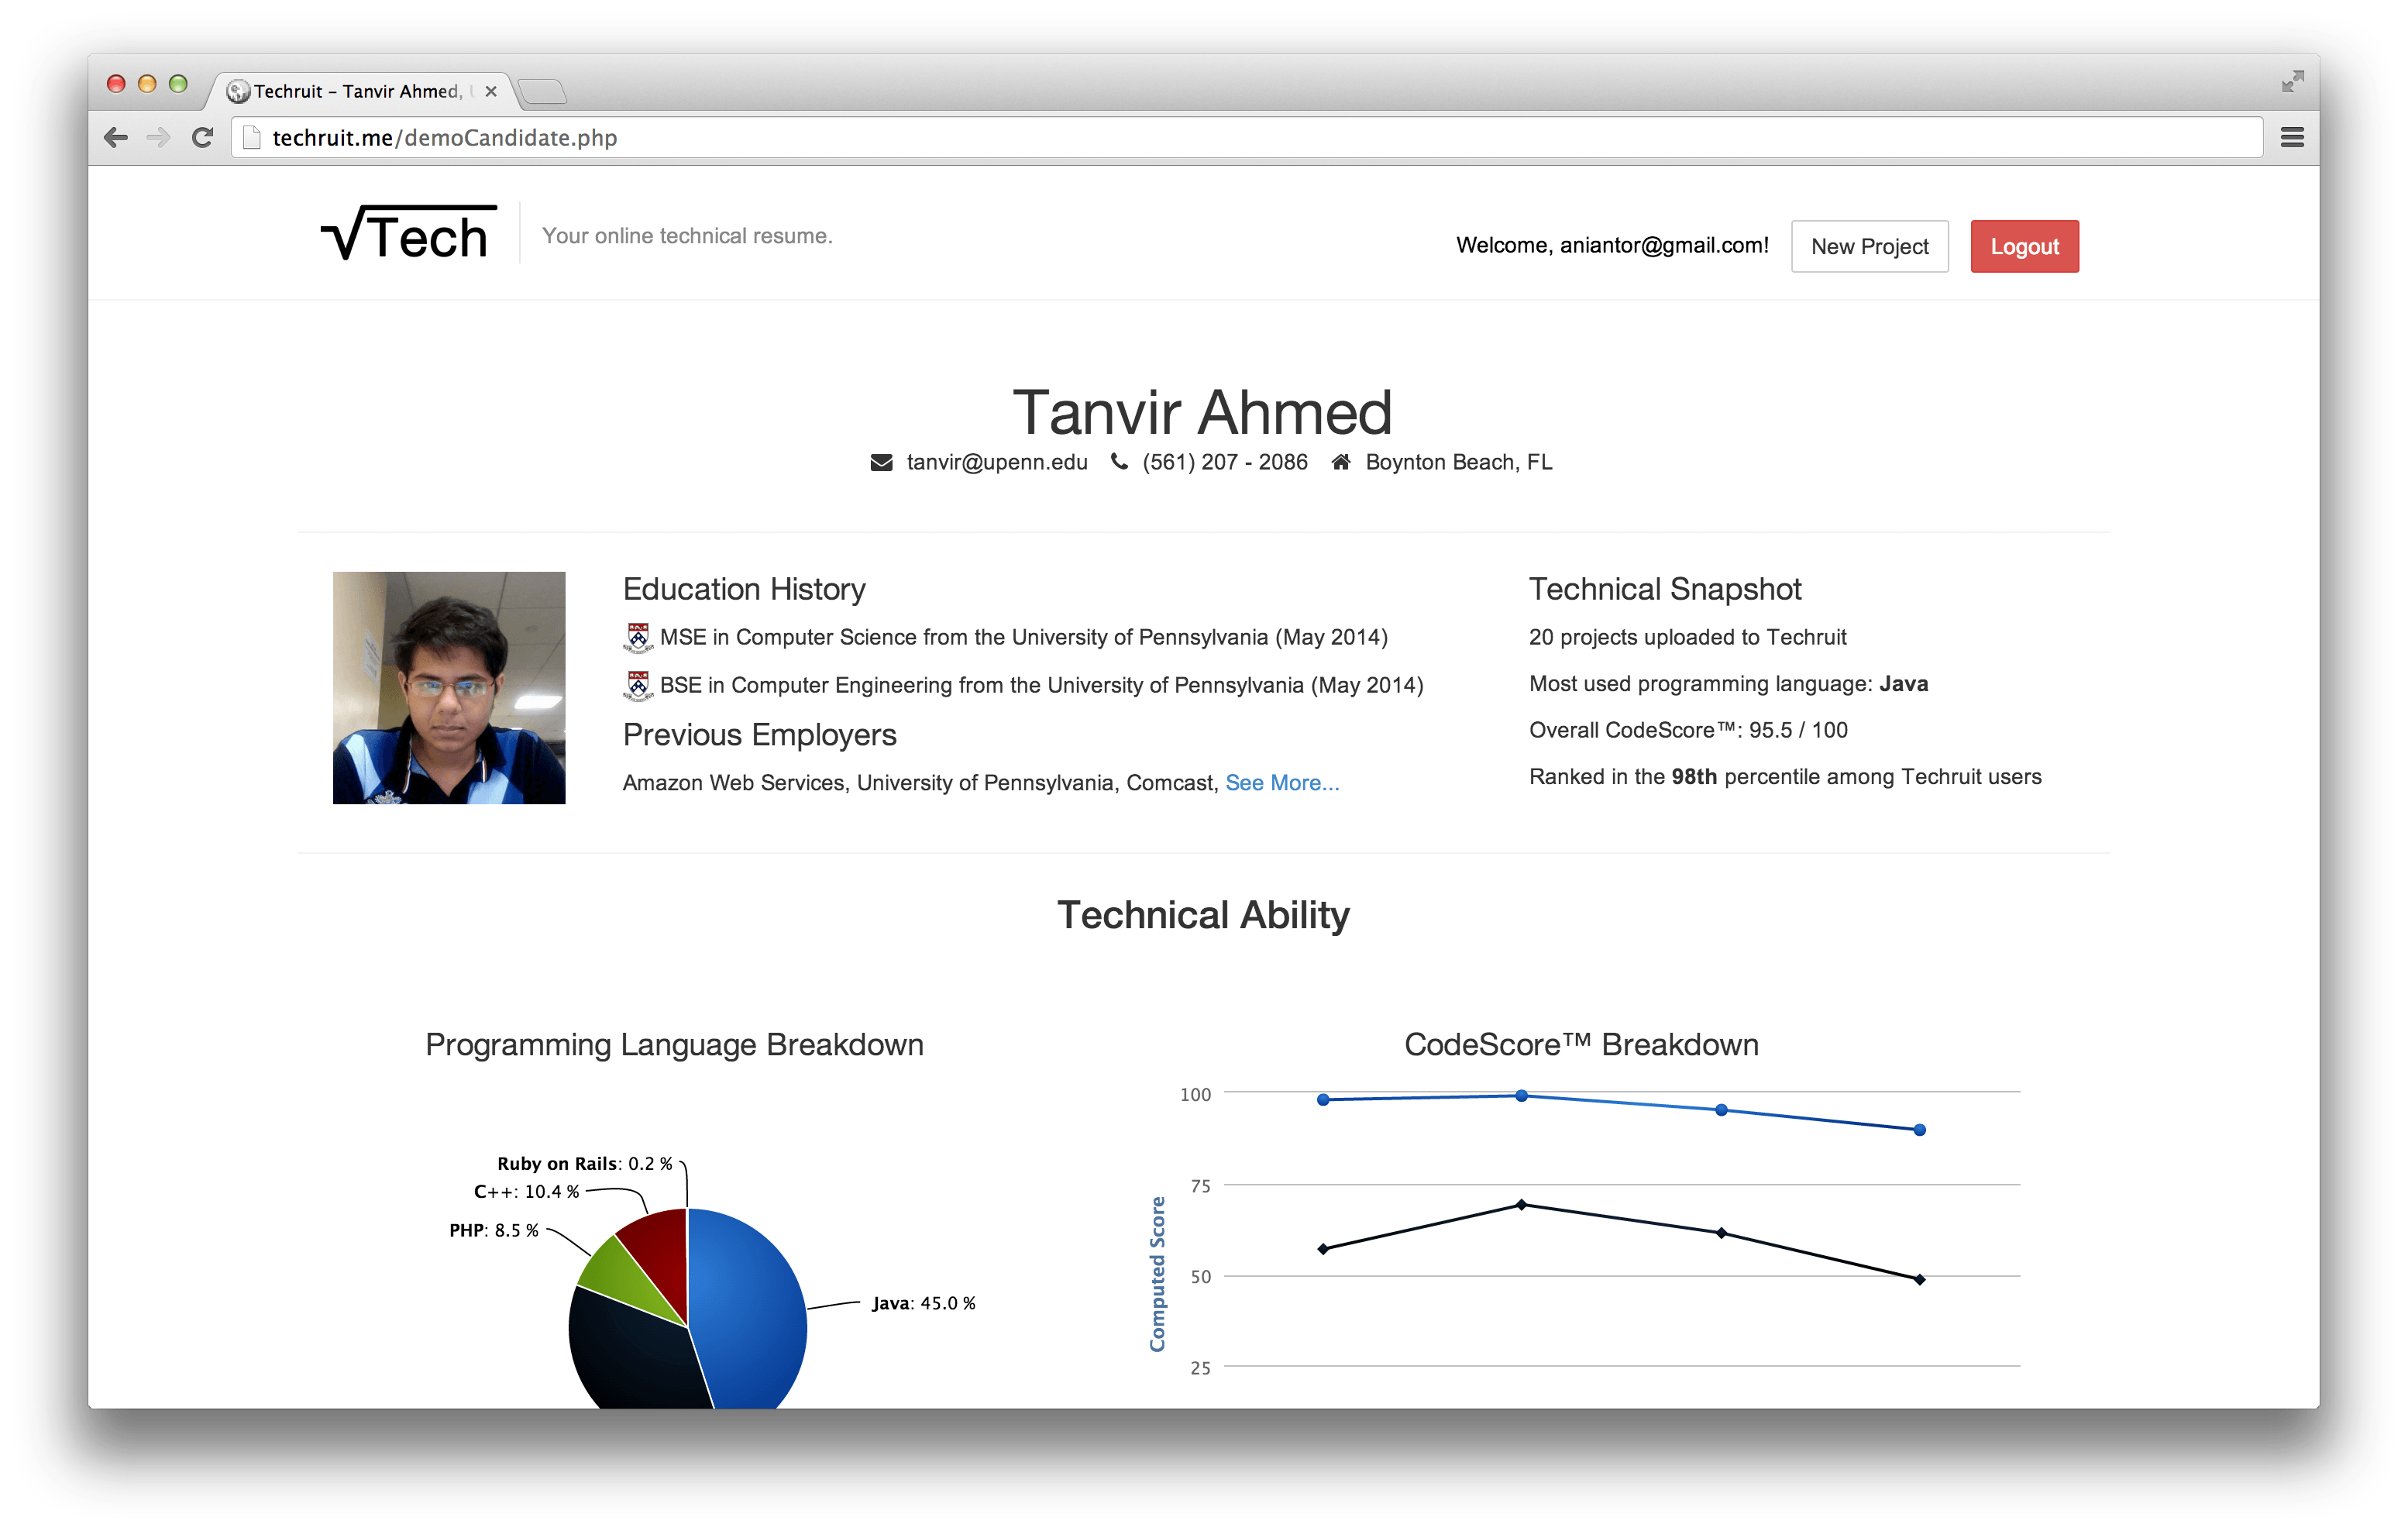
\includegraphics[width=500px]{sample_candidate}
	\end{center}
	\vspace{-12pt}
	\caption{Sample Candidate Profile}
	\label{fig:candidate}
\end{figure}

% We then use appendices to share some additional information with
% you, though you won't need appendices in your own proposal.

% The usage of 'enumerate' (similar to 'itemize') we talked about
% above

% You may also notice we have many 'vspace' commands lying
% around. These create 'vertical space' and are a way to force LaTeX
% to cooperate, sometimes. Don't get too involved with using them
% initially, though, because adding or deleting a single line of task
% can dramatically change how LaTeX chooses to format, page, and space
% the document
\end{document} 

